\chapter{Leaf Identification}

\section{Introduction}
In this chapter we discuss the mechanics of leaf classification exploring two different approaches and evaluating the success or otherwise of both.

For this stage of the project it is more productive to develop the vision software using Java SE on the desktop instead of in the Android environment. Because the OpenCV API will be used it is easy to port the techniques to Android after they are proven. This should offer an easier development path as we don't have to manage the extra level of complexity involved in deploying to a virtual or physical environment. 


\section{Algorithmic Approach}

This approach revolves around extracting certain features from an image, such as edges, colour, textures, contours, etc. and creating a model to match that leaf type.

It is important to keep the number of transformations performed on the individual image minimal as this project is targeting a resource starved environment. The Android application will also be required to display a number of frames per second to provide a sense of real-time feedback to the user, although this may be achieved by processing only every second or third frames.

In this section we will concentrate primarily on identifying shapes, which removes the necessity to store and manipulate large sized images and colour information. 

The concept being tested in this section is to perform a series of transformations to differentiate the leaf from the background, this is hoped to enhance the leaf’s edges for a given frame and finally using contours attempt to extract the shape of the leaf. 

\subsection{Resource Utilisation}

Early in the process we can combine the BGR (Blue, Green, Red) colour channels into a single grayscale channel and we may also sub-sample the image. These two optimisations will help minimise both CPU and memory utilisation.

Just to briefly describe the the gain from converting and storing the image in grayscale, we will analyse how the image is stored in OpenCV. The IplImage type that OpenCV operates with stores an image as a number of bitmaps, one for each channel of color information. For this project we define that each pixel will have a color depth of 255 separate colors and this is stored in a 8bit unsigned structure, giving 1 byte per pixel \cite{morganIPL06}.

For the video stream being analysed in the test environment the camera is returning an image size of 640 x 480 pixels and 3 channels of colour which is 307,200 pixels by 3 channels giving 921,600 pixels which is 921,600 bytes or 900 kilobytes per frame.  If we are to convert the image to a single channel we are now dealing with 307,200 pixels which is equivalent to 300 kilobytes per frame. This equates to a considerable memory saving, especially when we see as many as 24 frames per second being processed by OpenCV.

The actual image size returned depends on the model of the device, for example the device being used for this project is the Google Nexus One which is capable of capturing 720 x 480 pixels at 20 frames per second.

This analysis slightly simplistic as the IplImage type contains padding and metadata, but gives a good indication of the savings involved.

At this stage we are unable to provide an analysis of memory savings from sub-sampling performed on the image, as the optimal size for shape analysis is yet to be discovered.


\subsection{Preparing the Image}

Once an frame is retrieved from the camera’s sensor we must preprocess the image before attempting to classify features contained in the image. The goal of preparing the image is twofold, firstly we need to perform filtering to the image in order to separate the foreground objects from the background, and secondly the \emph{cvFindContours()} function requires a binary image as input.

The order and configuration of these transforms that are applied to the frames are determined through much experimentation, until reasonable  results are achieved. Below we describe the transformations and the order in which they are utilised.

\begin{figure}
\centering
    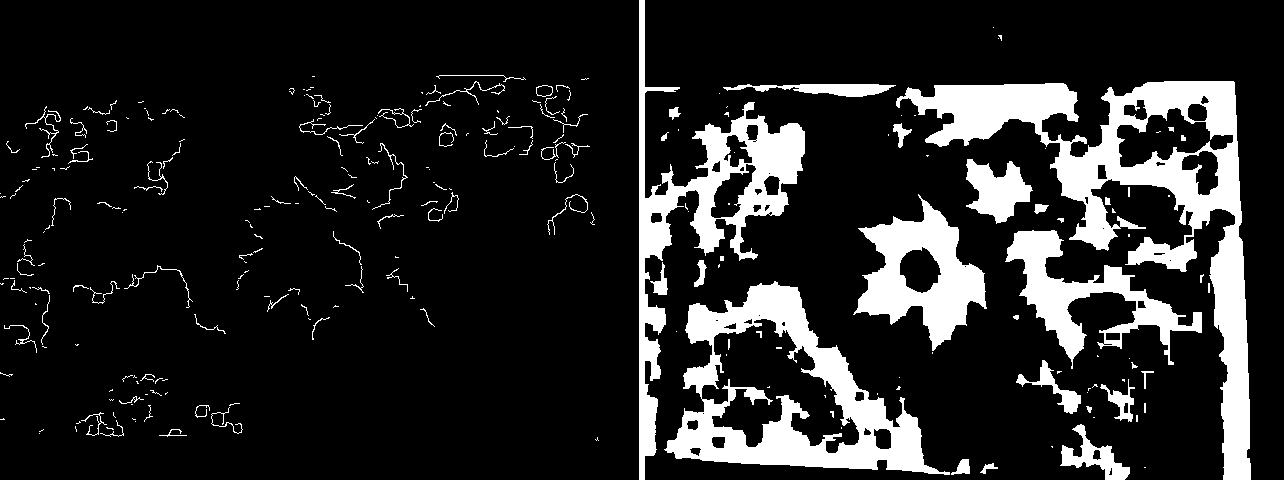
\includegraphics[width=1.0\textwidth]{leaf_identification/images/convert_to_binary.png}
    \caption{Binary image conversion, Canny Edge detection (left) and Adaptive Threshold (right)}%
    \label{preprocessing}
    \colorbox{red}{replace with example of each stage}
\end{figure}


\subsubsection{Convert to grayscale}
As discussed earlier we attempt to optimise any processing by minimising both the memory and CPU utilisation. As colour information is unnecessary for this approach we remove it at the first available opportunity.

It would be also advisable at this stage to sub-sample the image to the smallest size possible while still achieving good matches.

\subsubsection{Histogram Equalization}
The image quality from mobile phone sensors vary widely, but one common problem that would hinder the classification of shapes in an image is the lack of contrast. With histogram equalisation we redistribute brightness across the range of the image, expanding the dynamic range of the image which increases the contrast \cite{kuntz09}.


\subsubsection{Threshold}
When applying a threshold filter to an image we are essentially making a decision to accept or reject a particular pixel based on a certain threshold value \cite{bradski08}. OpenCV provides a number of options for how the threshold is to be calculated, after experimentation it was found that adaptive threshold offered the best results.

Adaptive threshold is a technique where the threshold value is variable, this threshold value is calculated as a weighted average from a predetermined pixel region around the current pixel.

Once this transform is applied to the input image we are returned a binary version of that image which can then be used to find contours, we will discuss this further in the next section.


\subsubsection{Dilate}
Once the image has been converted to a binary image, we apply a dilate transform to help minimise small clusters of pixels which may have not met the threshold in the middle of an identified shape. Applying the filter at this stage helps to provide a binary image with cleaner more identifiable shapes to the next stage of processing.


\subsubsection{Other techniques}
After experimenting with a number of different techniques for creating a good quality binary representation of the raw image, the procedure outlined above was finalised on. But a number of other approaches are also quite valid and provide reasonable results, these include the use of Canny Edge detection, background subtraction and Sobel operators.


\subsection{Identifying features}

\colorbox{red}{replace with example of each stage}

As seen in Figure \colorbox{red}{binary image}, we should now provided with a clean binary image of any objects captured by the sensor. We must now use some mechanism to capture the detected shapes and compare them to a store of pre-captured shapes in an efficient manner. 

\subsubsection{Contours}
OpenCV provides a useful function called \emph{cvFindContours()} which maps boundaries in a binary image. A contour is a list of points that represent, a curve in an image \cite{bradski08}. We must be aware that the contours we are returned are those discovered in the image and due to lighting and other conditions may not represent the actual object.

The function returns a contour tree which describes the nested structure of all the contours found. This concept of which contour contains another maybe useful for certain forms of shape analysis. A individual contour is returned as a sequence of \emph{(x, y)} points that describe the edge of an object.


\subsubsection{Polygon Approximations}
Returned contours are are quite specific to the detected shape, which is heavily dependant on lighting conditions and other such external interferences. We apply a Polygon Approximation to the contour which helps to create a more generic representation of the shape correcting for defects in the image and the physical leaf. This also has the added advantage of minimising the number of points on the curve which decreases the signature of the shape, this is helpful later when storing the shape.

\subsubsection{Shape Matching}
OpenCV provides a function called \emph{cvMatchShapes()} which compares two shapes and determines if they are similar. This function matches the shapes using Hu Moments which we will talk about in a moment and returns a double indicating how closely the shapes match with 0.0 being a match.

From exposing many different silhouettes of leaves a value of less than 0.2 can be considered to be a good match. However it is likely that with a larger database of leaf types to match against a more precise match may be required.


\subsection{Storage and Retrieval}
Possible to store grayscale image of each leaf and compare with cvMatchShapes but his would be very inefficent and not a viable solution for the project. (template matching - http://nashruddin.com/template-matching-in-opencv-with-example.html)
\section{Machine Learning Approach}
